% This file was created with tikzplotlib v0.10.1.
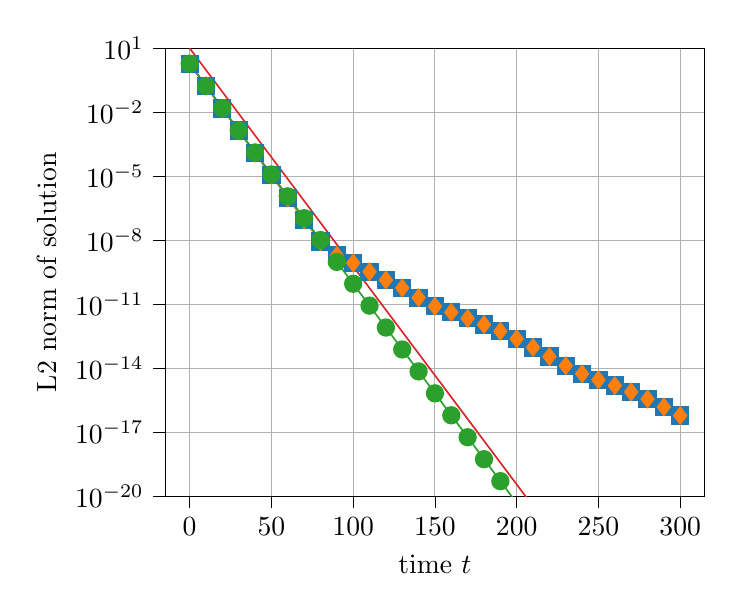
\begin{tikzpicture}

\definecolor{crimson2143940}{RGB}{214,39,40}
\definecolor{darkgray176}{RGB}{176,176,176}
\definecolor{darkorange25512714}{RGB}{255,127,14}
\definecolor{forestgreen4416044}{RGB}{44,160,44}
\definecolor{steelblue31119180}{RGB}{31,119,180}

\begin{axis}[
log basis y={10},
tick align=outside,
tick pos=left,
x grid style={darkgray176},
xlabel={time $t$},
xmajorgrids,
xmin=-15, xmax=315,
xtick style={color=black},
y grid style={darkgray176},
ylabel={L2 norm of solution},
ymajorgrids,
ymin=1e-20, ymax=10,
ymode=log,
ytick style={color=black},
ytick={1e-23,1e-20,1e-17,1e-14,1e-11,1e-08,1e-05,0.01,10,10000},
yticklabels={
  $\mathdefault{10^{-23}}$,
  $\mathdefault{10^{-20}}$,
  $\mathdefault{10^{-17}}$,
  $\mathdefault{10^{-14}}$,
  $\mathdefault{10^{-11}}$,
  $\mathdefault{10^{-8}}$,
  $\mathdefault{10^{-5}}$,
  $\mathdefault{10^{-2}}$,
  $\mathdefault{10^{1}}$,
  $\mathdefault{10^{4}}$
}
]
\addplot [semithick, steelblue31119180, mark=square*, mark size=3, mark options={solid}]
table {%
0 1.87090036052962
10 0.174489326028517
20 0.0150975771261266
30 0.00138003358268177
40 0.000118941546226639
50 1.1099739590041e-05
60 9.6475313927122e-07
70 9.27083588448855e-08
80 8.88205767686982e-09
90 1.95339247587347e-09
100 8.64750024347657e-10
110 3.3726878085795e-10
120 1.37499552767375e-10
130 5.82527393564931e-11
140 2.05269641434267e-11
150 8.07885275258263e-12
160 4.22232261546628e-12
170 2.20871881154813e-12
180 1.12897126002079e-12
190 5.47970139844139e-13
200 2.41756902710079e-13
210 9.54580259926548e-14
220 3.55566035833886e-14
230 1.32218697840379e-14
240 5.57379073906199e-15
250 2.89824069170654e-15
260 1.55886893548118e-15
270 7.84337172977893e-16
280 3.64878335574703e-16
290 1.56313177050692e-16
300 6.14224846992793e-17
};
\addplot [semithick, darkorange25512714, mark=diamond*, mark size=3, mark options={solid}]
table {%
0 1.87090036052962
10 0.173782760646898
20 0.0150255167798845
30 0.00137910198965973
40 0.000120086755373626
50 1.12359180125779e-05
60 9.76357254535007e-07
70 9.23992531840376e-08
80 8.82010573210179e-09
90 1.94702066800678e-09
100 8.6452489028425e-10
110 3.37298881500433e-10
120 1.37506739379973e-10
130 5.82608186806785e-11
140 2.05282381041008e-11
150 8.0790557816388e-12
160 4.2226205646461e-12
170 2.20885467457475e-12
180 1.12898495074389e-12
190 5.47971263124361e-13
200 2.41761304434991e-13
210 9.54605962811564e-14
220 3.55573218751175e-14
230 1.32220614329006e-14
240 5.57386837743307e-15
250 2.89828128857421e-15
260 1.5588884580492e-15
270 7.84341866966862e-16
280 3.64879205018774e-16
290 1.56313612827154e-16
300 6.14228363426435e-17
};
\addplot [semithick, forestgreen4416044, mark=*, mark size=3, mark options={solid}]
table {%
0 1.87090036052962
10 0.167906622547116
20 0.0152547158371657
30 0.00140243380228884
40 0.000130271657311899
50 1.21996641201202e-05
60 1.14899386812342e-06
70 1.08585155527167e-07
80 1.02774382718609e-08
90 9.72839436261965e-10
100 9.20053398256894e-11
110 8.68841191975079e-12
120 8.19025657310313e-13
130 7.70661542908942e-14
140 7.23934557421525e-15
150 6.79088664589721e-16
160 6.36375010784999e-17
170 5.96016805754538e-18
180 5.58185862152816e-19
190 5.22987905372147e-20
200 4.90454962230999e-21
210 4.60543985832032e-22
220 4.33141290181463e-23
230 4.08072338606358e-24
240 3.85116042992489e-25
250 3.64022180393027e-26
260 3.44530068265139e-27
270 3.26386468804083e-28
280 3.0936090087328e-29
290 2.93257059974141e-30
300 2.77919717615354e-31
};
\addplot [semithick, crimson2143940]
table {%
0 10
10 0.951111830888997
20 0.090461371485702
30 0.00860388806584957
40 0.000818325973107418
50 7.78319514546217e-05
60 7.40268898496687e-06
70 7.04078507399366e-07
80 6.69657398262203e-08
90 6.36919074129526e-09
100 6.05781266723458e-10
110 5.76165729711604e-11
120 5.47998042081499e-12
130 5.2120742112772e-13
140 4.95726544581719e-14
150 4.71491381437395e-15
160 4.48441031047303e-16
170 4.2651757008515e-17
180 4.05665906990013e-18
190 3.85833643526517e-19
200 3.66970943113078e-20
210 3.49030405587341e-21
220 3.31966948094105e-22
230 3.15737691796417e-23
240 3.00301854125156e-24
250 2.85620646296337e-25
260 2.71657175838608e-26
270 2.58376353885993e-27
280 2.45744807002931e-28
290 2.3373079332002e-29
300 2.22304122769743e-30
};
\end{axis}

\end{tikzpicture}
